\section{\benchmark{}}

\subsection{Design Goals}

\benchmark{} aims to measure whether an autonomous agent can learn from experience in an unfamiliar real world environment. This requires two properties from a benchmark that existing evaluations lack:

\begin{itemize}
    \item \textbf{Ultra-long-horizon, diverse tasks.} Learning behaviors such as exploration, strategy revision, and experience accumulation need time and complexity to emerge. Short tasks are usually solved from memory rather than learning, so measuring learning calls for long-horizon tasks. Because learning is a general capability, these tasks must also span diverse domains.
    \item \textbf{Realistic, multi-level feedback.} In practice, human experts learn from rich feedback: test failures, experimental results, unexpected phenomena, authoritative judgments, and more. A benchmark that cannot offer such rich feedback cannot measure learning, and leaves the agent guessing what the evaluation actually rewards. We need feedback that approximates the real world, so we can measure true, general-purpose learning.
\end{itemize}

The first requirement motivates our task taxonomy (\S\ref{sec:taxonomy}): 134 tasks across six capability families, each designed as a day-scale challenge that supports frontier models running for at least 12 hours. The second motivates our evaluation protocol (\S\ref{sec:evaluation-protocol}): each task individually simulates its own slice of the real world, providing isolated work and judge environments, local agent-driven feedback, submission-gated judge feedback, and host-side trajectory measurement.

\subsection{Task Taxonomy}
\label{sec:taxonomy}

We searched for real world tasks that satisfy two criteria: a performance ceiling high enough that no current agent can saturate it, and a workflow that supports continuous learning rather than one-shot completion. This search, conducted in collaboration with domain experts across fields, identified six capability families and yielded 134 curated tasks (Figure~\ref{fig:taxonomy}):

\begin{itemize}
    \item \textbf{Scientific Problems \& ML} (39 tasks). Each task uses real world research data and experimental settings sourced from working scientists. Domain expertise is essential: agents must formulate hypotheses, choose models, validate against noisy observations, and refine iteratively. Many problems are open-ended, with no known optimal solution.

    \item \textbf{Systems \& Software Engineering} (36 tasks). Agents work on production-grade codebases where a single task may require thousands of lines of change, with over 100{,}000 lines in the largest cases. Because the code spans interdependent modules, an agent must reason about cross-module coupling while meeting both correctness and performance targets.

    \item \textbf{Combinatorial Optimization} (19 tasks). These are open-ended, predominantly NP-hard problems where exact methods are intractable and progress depends on designing, tuning, and iterating on heuristic search strategies. Even strong solvers have room to improve with additional time and feedback.

    \item \textbf{Professional Knowledge Work} (19 tasks). These tasks reproduce real white-collar deliverables across finance, education, healthcare, and legal domains, matching work that would take a human professional with three or more years of experience roughly three full days to complete. Many tasks feature carefully designed rubrics and multi-round delivery feedback that approximate real client review cycles, so agents can learn from structured critique and revise iteratively.

    \item \textbf{Formal Math \& Theorem Proving} (13 tasks). These tasks sit at the frontier of mathematical difficulty and require building large-scale machine-checked proofs in Lean, coupling deep mathematical insight with substantial formal-verification engineering. Most are newly created for \benchmark{} and designed to support iterative progress: agents receive structured intermediate guidance and can extend partial proofs incrementally.

    \item \textbf{Interactive Games \& Simulators} (8 tasks). These are real games designed for human players, where proficient humans typically invest tens of hours to master the mechanics. The state spaces are enormous and each run is procedurally distinct, so agents face strong out-of-distribution pressure. Agents must develop and refine strategies through high-frequency interaction across many episodes.
\end{itemize}

Tasks whose primary difficulty lies in visual understanding, especially GUI operation, are excluded. When success depends on the vision backbone rather than iterative reasoning, learning ability and perceptual capability are hard to separate.

\subsection{Feedback Loop and Evaluation Protocol}
\label{sec:evaluation-protocol}
\label{sec:feedback-design}

\begin{figure}[!t]
\centering
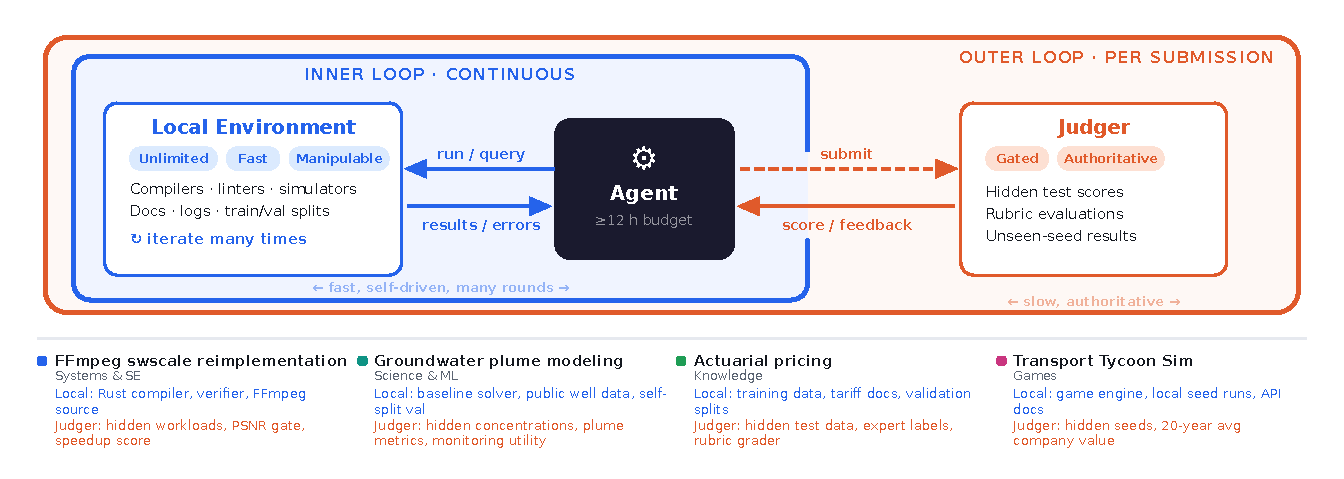
\includegraphics[width=\linewidth]{figures/fig_dual_loop.pdf}
\caption{The informative feedback loop in \benchmark{}. The inner loop (blue) lets agents iterate freely with local feedback; the outer loop (orange) gates authoritative judge feedback behind submissions. Bottom: representative tasks showing how both feedback channels are instantiated across capability families.}
\label{fig:dual-loop}
\end{figure}

\begin{figure}[p]
\centering
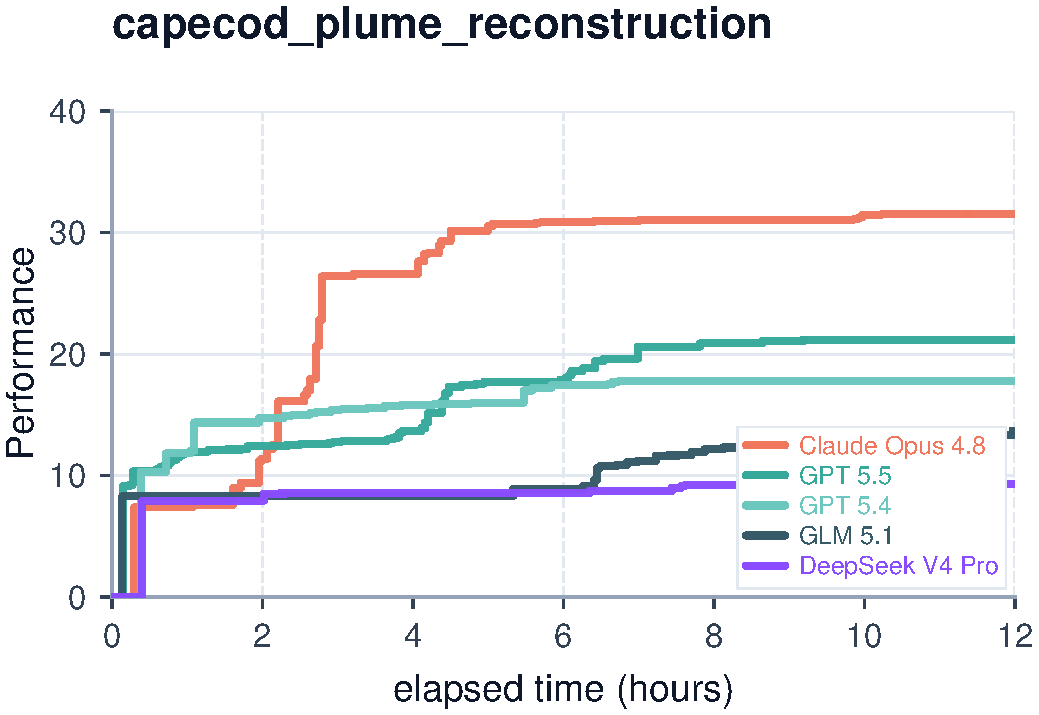
\includegraphics[width=0.31\linewidth]{figures/curves/capecod_plumebench_time_performance.pdf}\hfill
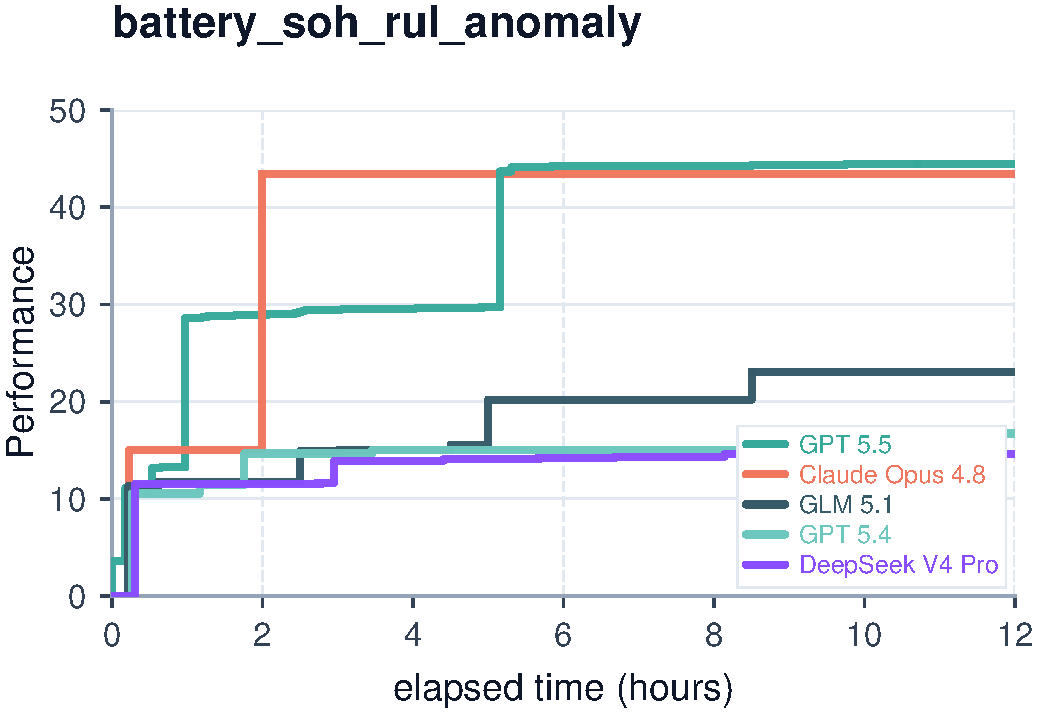
\includegraphics[width=0.31\linewidth]{figures/curves/battery_soh_rul_anomaly_time_performance.pdf}\hfill
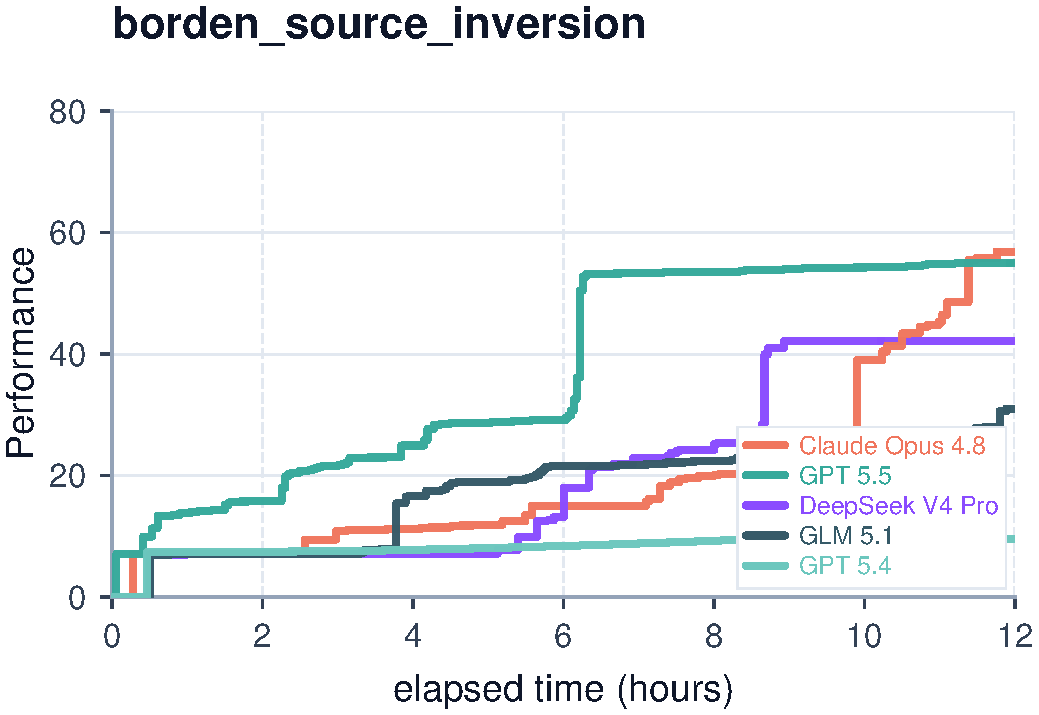
\includegraphics[width=0.31\linewidth]{figures/curves/borden_inverse_time_performance.pdf}

\vspace{0.05em}
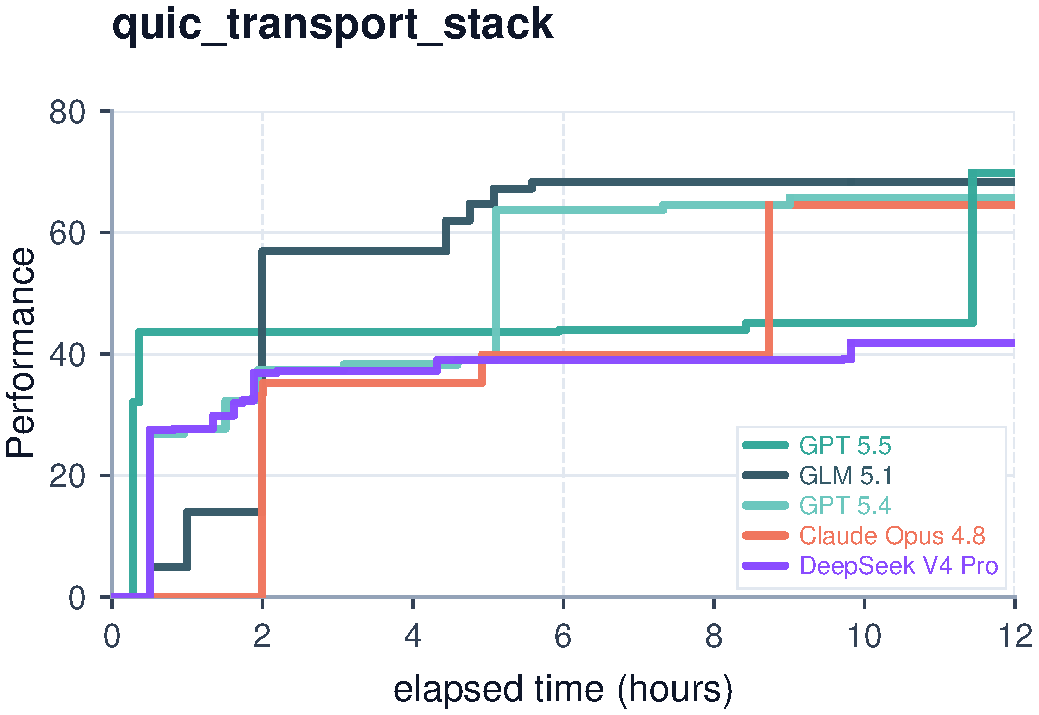
\includegraphics[width=0.31\linewidth]{figures/curves/quic_transport_stack_subset_time_performance.pdf}\hfill
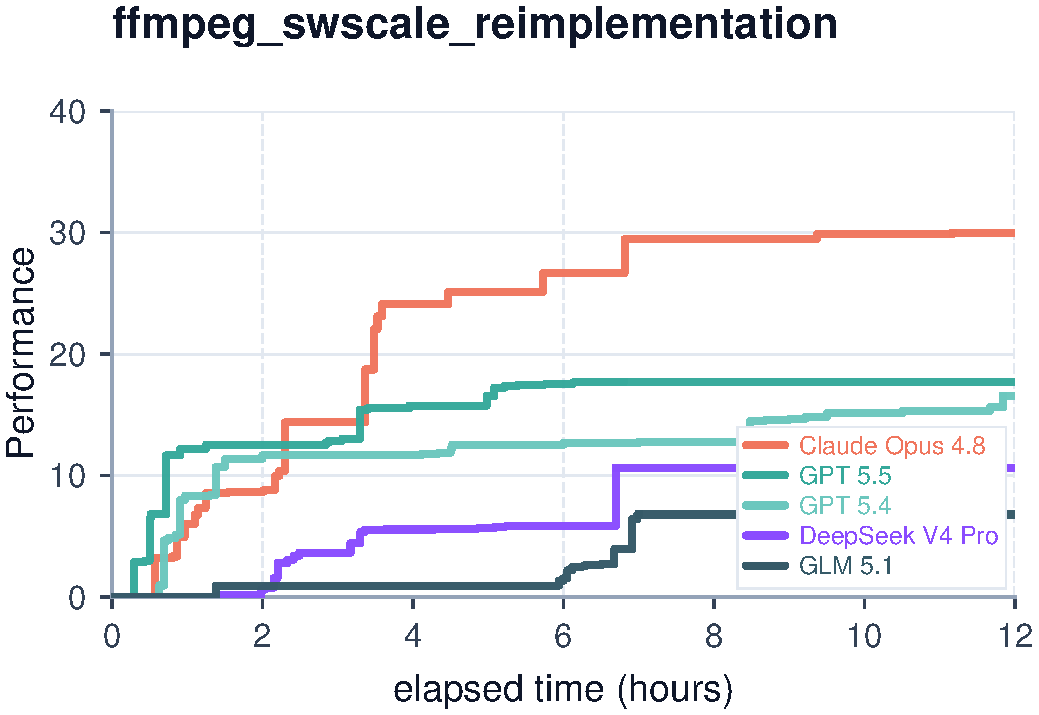
\includegraphics[width=0.31\linewidth]{figures/curves/ffmpeg_swscale_rewrite_time_performance.pdf}\hfill
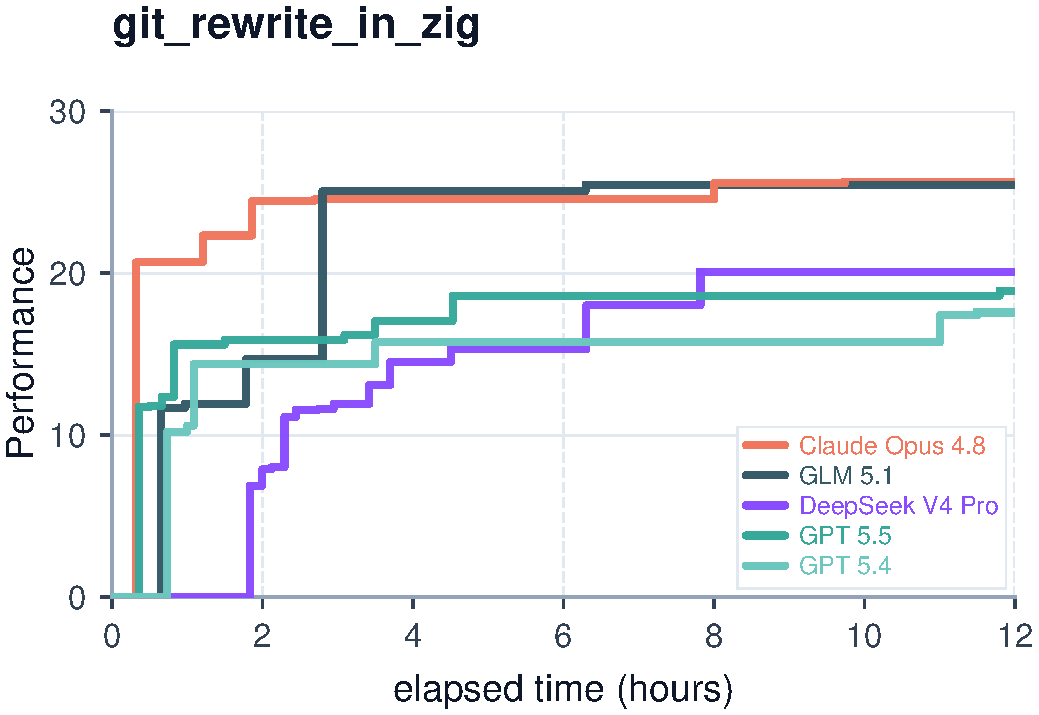
\includegraphics[width=0.31\linewidth]{figures/curves/git_to_zig_time_performance.pdf}

\vspace{0.05em}
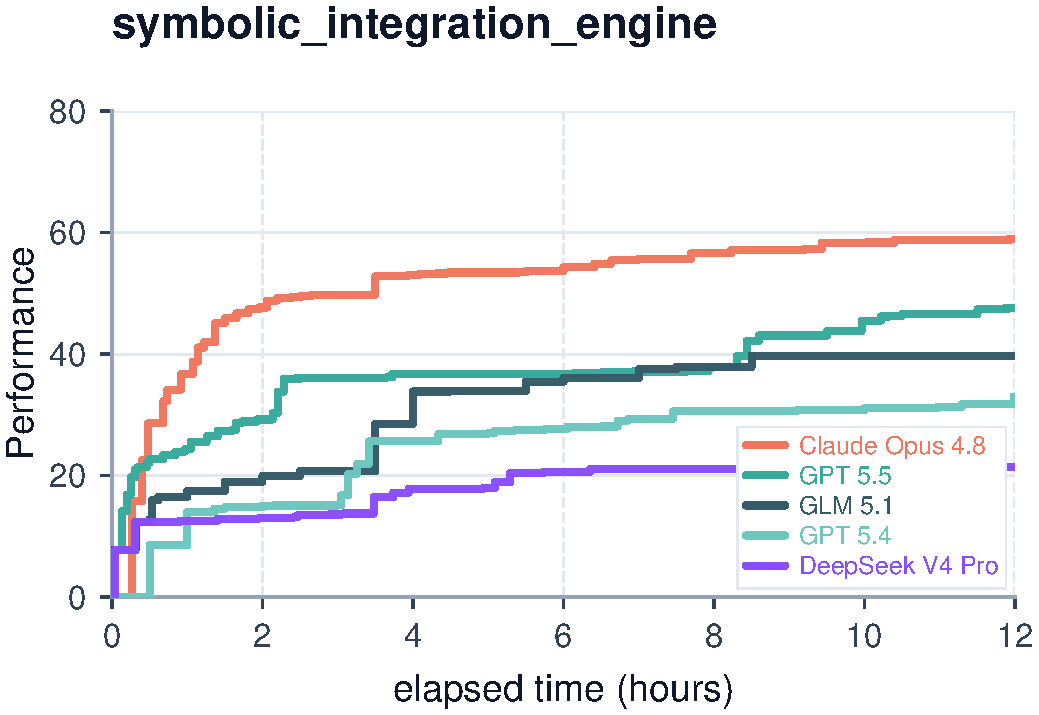
\includegraphics[width=0.31\linewidth]{figures/curves/symbolic_integration_engine_time_performance.pdf}\hfill
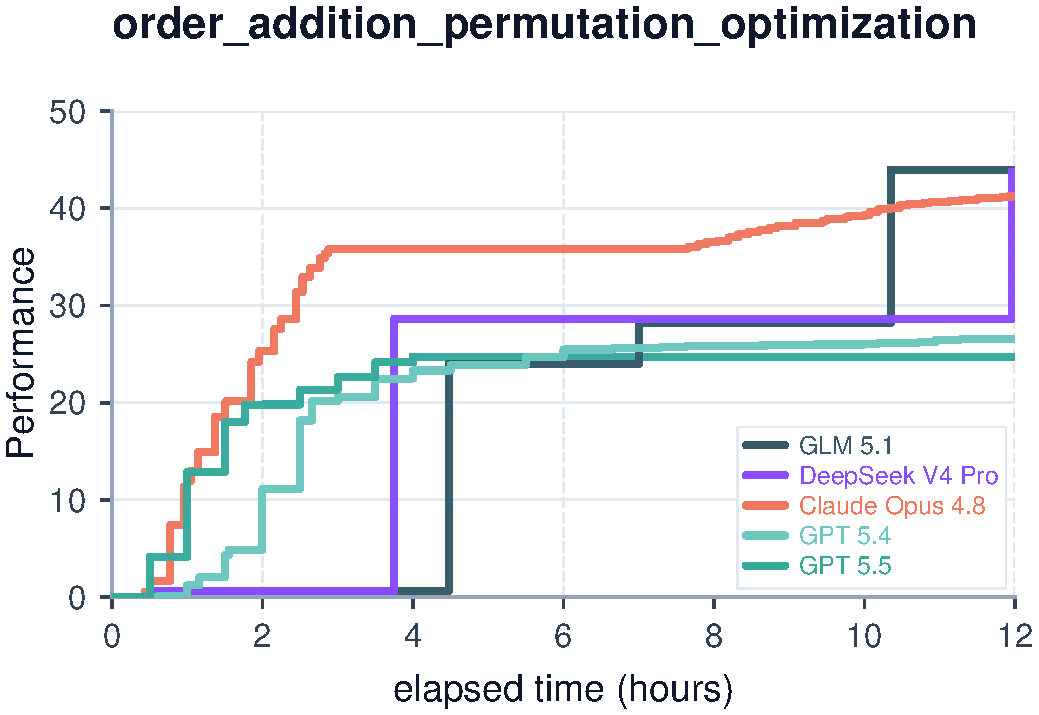
\includegraphics[width=0.31\linewidth]{figures/curves/complex_job_scheduling_time_performance.pdf}\hfill
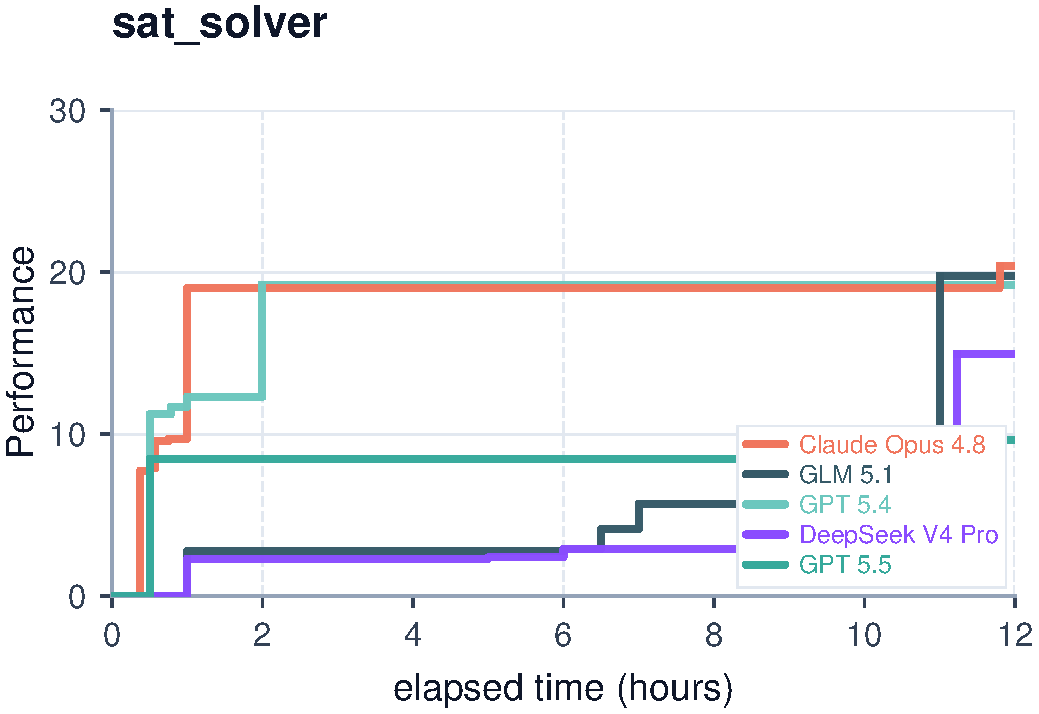
\includegraphics[width=0.31\linewidth]{figures/curves/sat_solver_time_performance.pdf}

\vspace{0.05em}
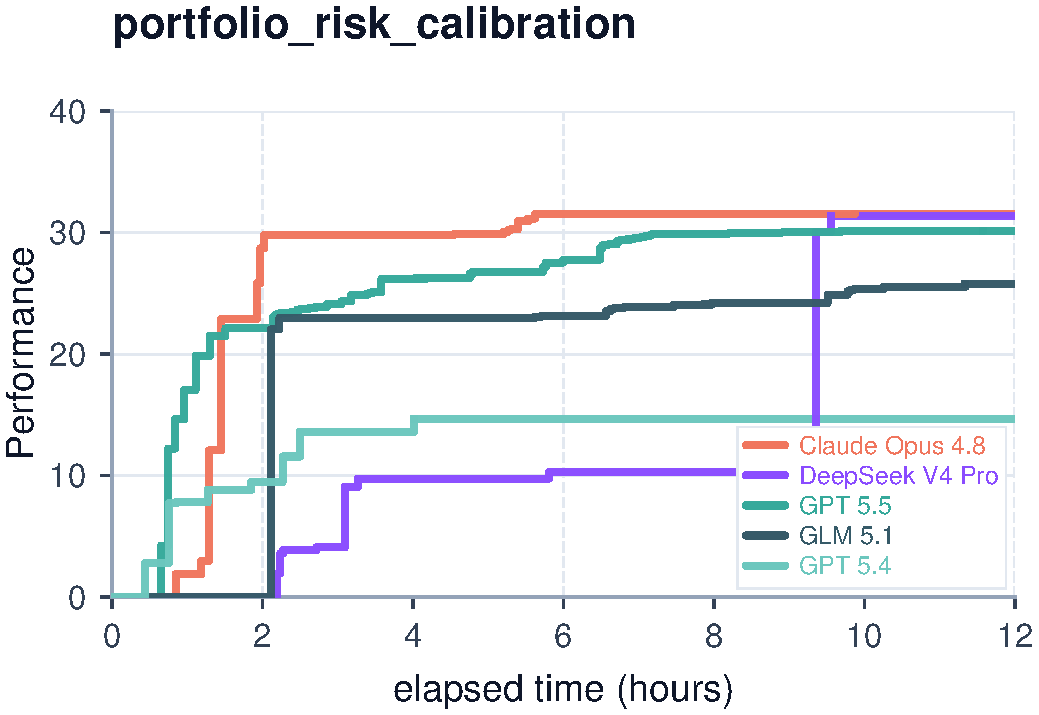
\includegraphics[width=0.31\linewidth]{figures/curves/adaptive_portfolio_risk_calibration_time_performance.pdf}\hfill
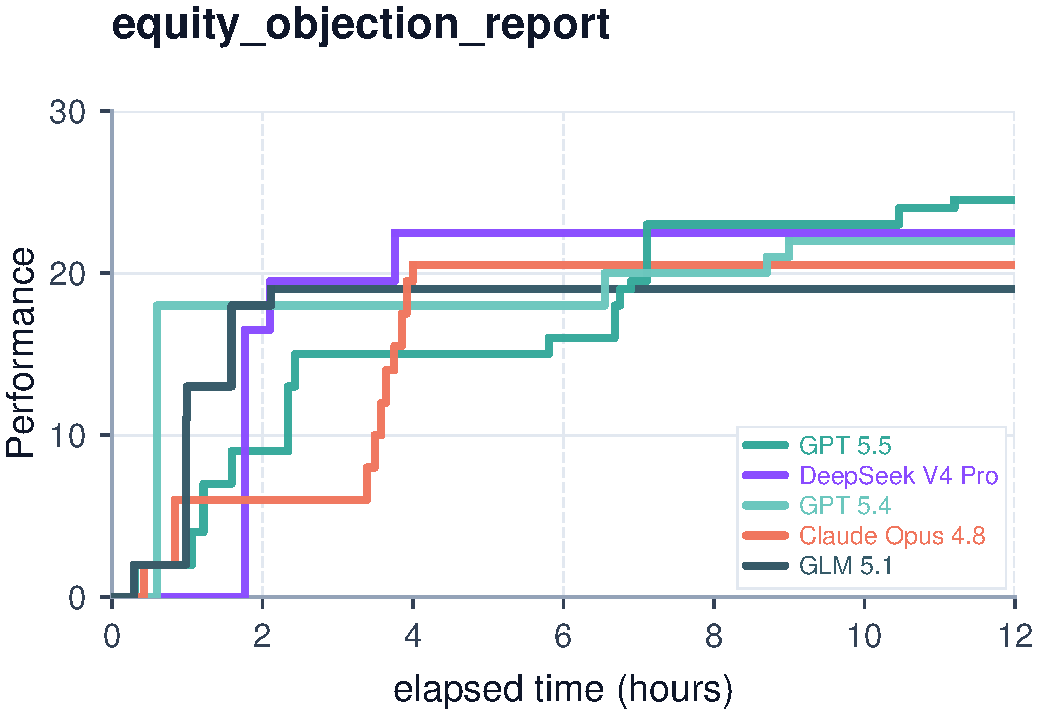
\includegraphics[width=0.31\linewidth]{figures/curves/equity_objection_report_time_performance.pdf}\hfill
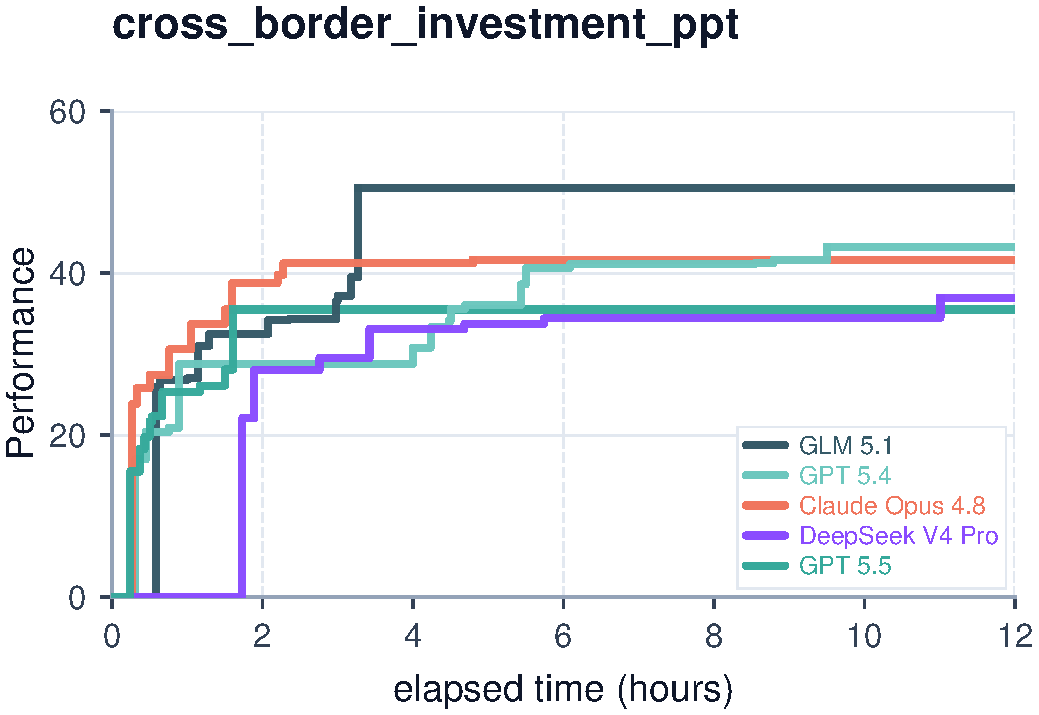
\includegraphics[width=0.31\linewidth]{figures/curves/cross_border_investment_policy_ppt_time_performance.pdf}

\vspace{0.05em}
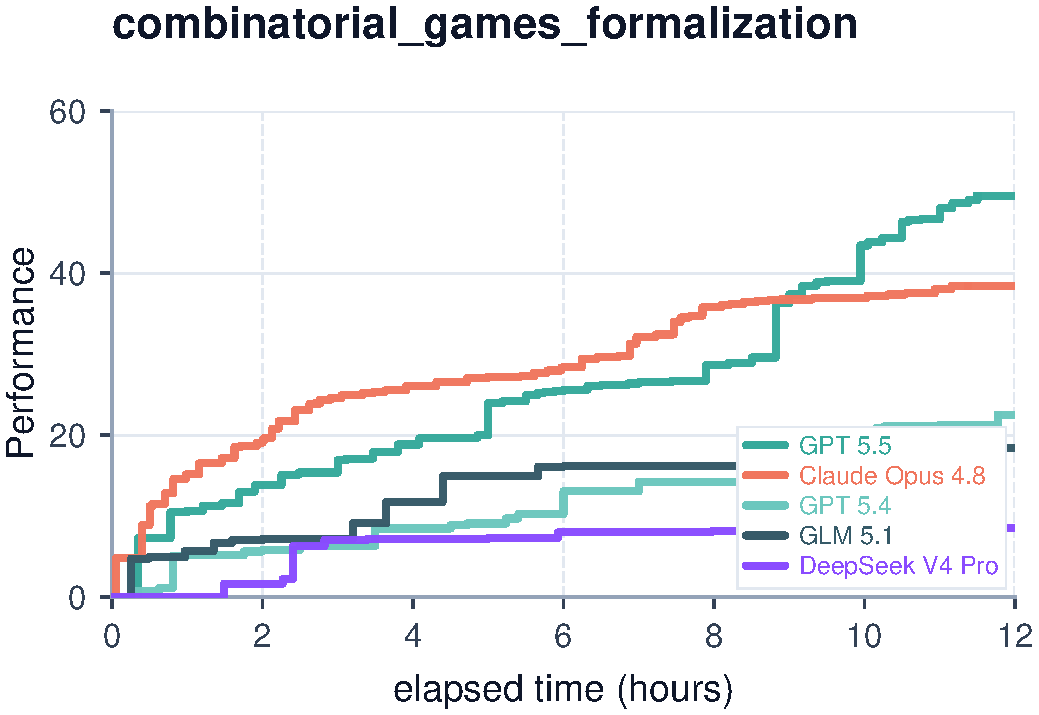
\includegraphics[width=0.31\linewidth]{figures/curves/combinatorial_time_performance.pdf}\hfill
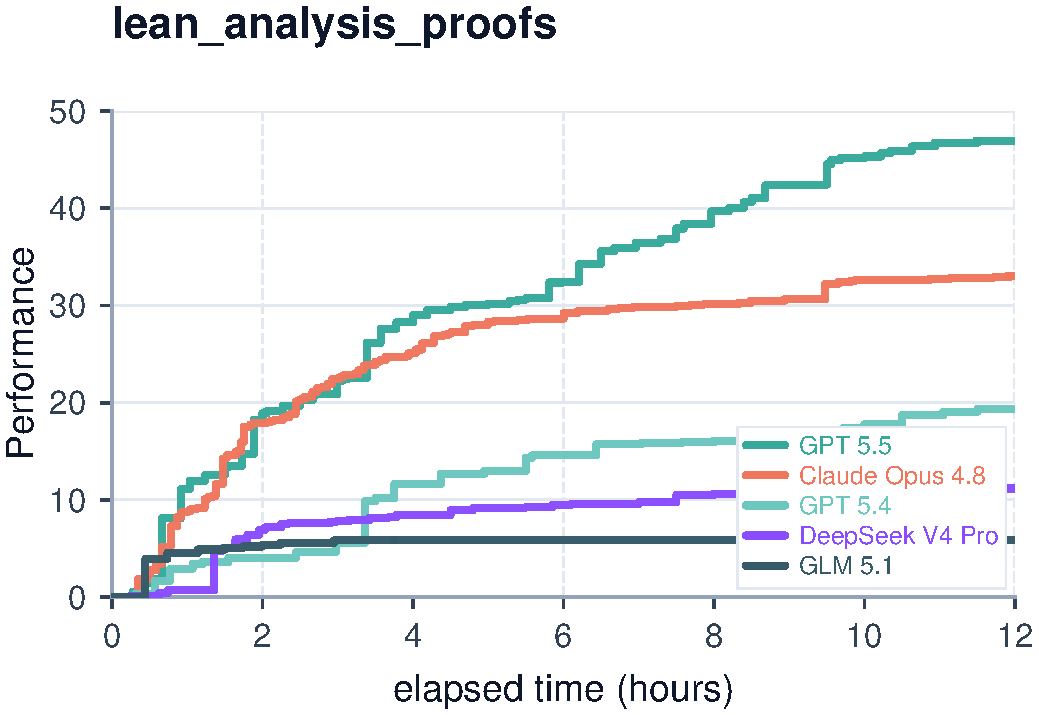
\includegraphics[width=0.31\linewidth]{figures/curves/analysis_time_performance.pdf}\hfill
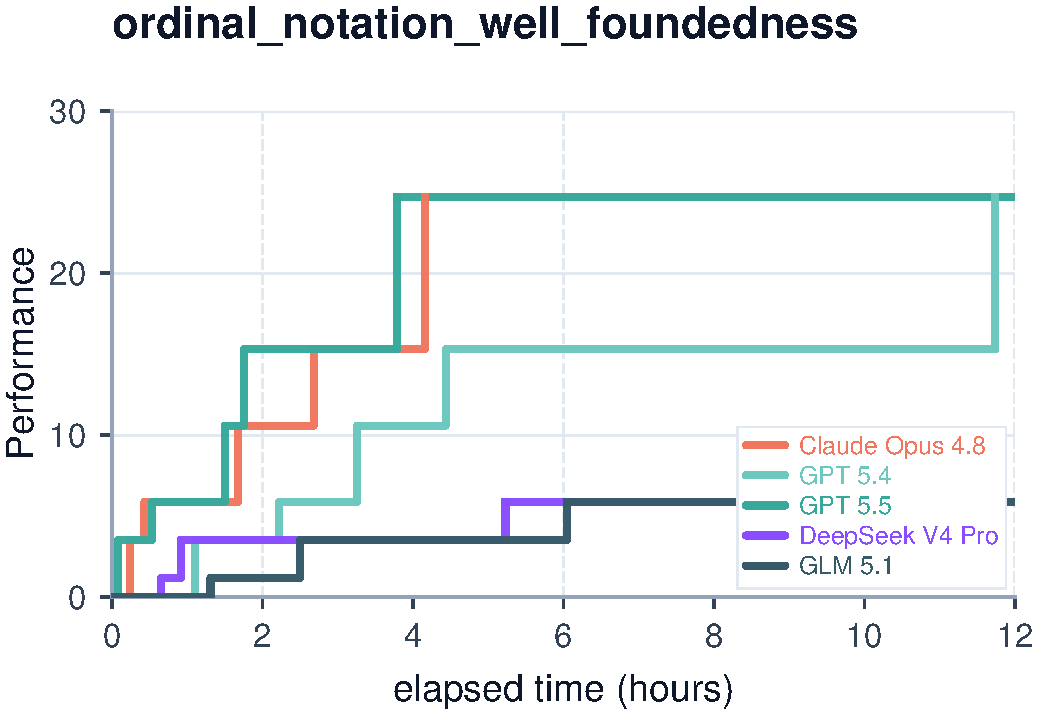
\includegraphics[width=0.31\linewidth]{figures/curves/ordinal_notation_wf_time_performance.pdf}

\vspace{0.05em}
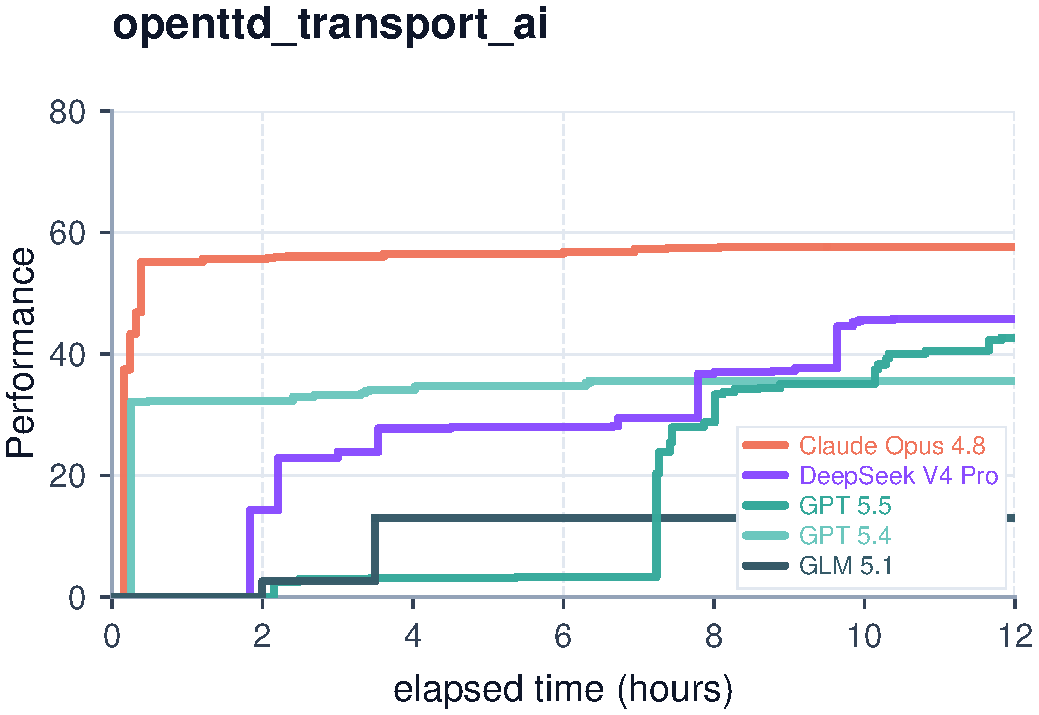
\includegraphics[width=0.31\linewidth]{figures/curves/openttd_time_performance.pdf}\hfill
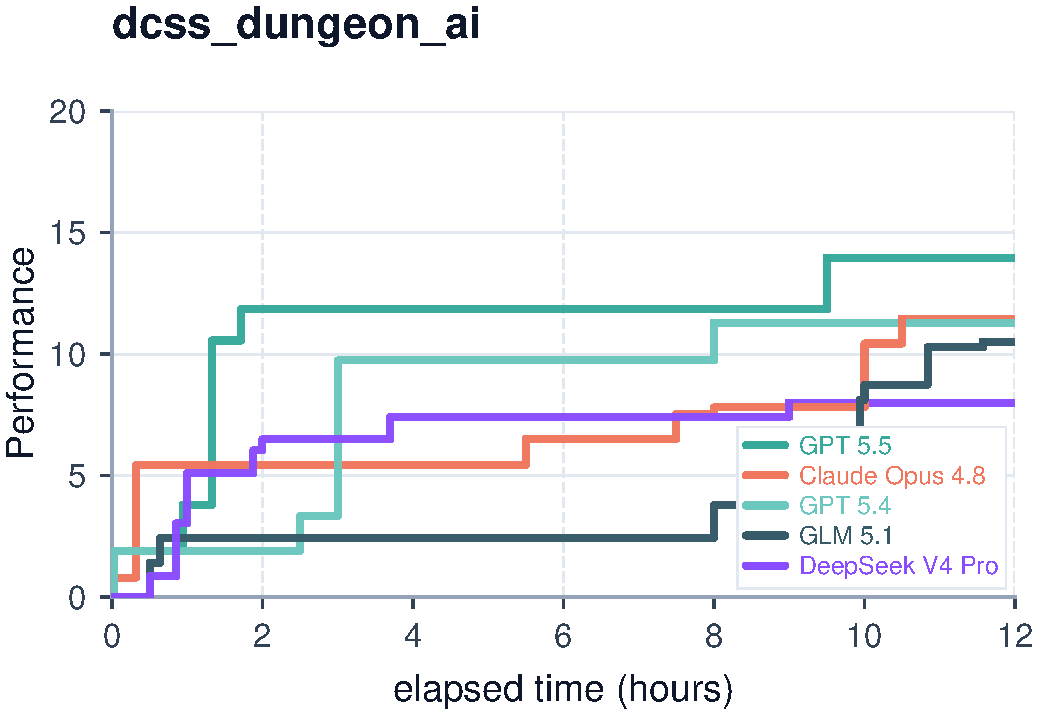
\includegraphics[width=0.31\linewidth]{figures/curves/dcss_time_performance.pdf}\hfill
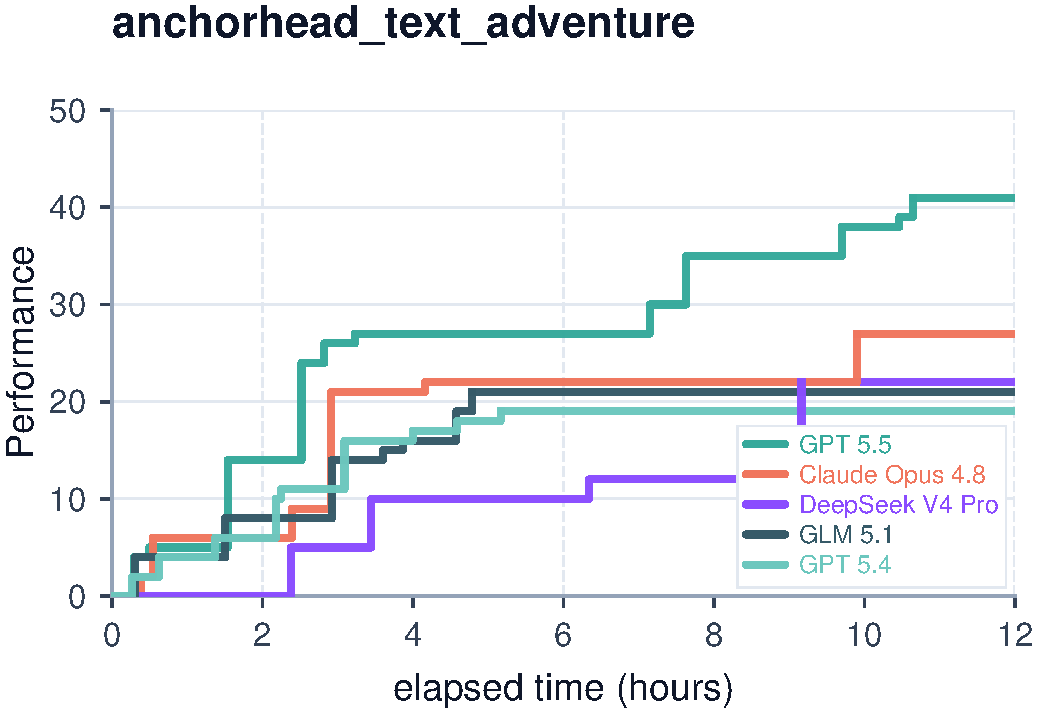
\includegraphics[width=0.31\linewidth]{figures/curves/jericho_anchorhead_time_performance.pdf}
\caption{Learning curves over 12 hours for 18 representative tasks across six capability families. The remaining task curves are provided in Figures~\ref{fig:curves-all-1}--\ref{fig:curves-all-21}.}
\label{fig:environment-data-curves-copy}
\end{figure}

Real world engineering and research workflows rarely provide a single final answer check. Instead, practitioners iterate through \textbf{two complementary feedback loops}: a fast local loop for exploration, debugging, and refinement, and a slower external loop that provides authoritative calibration through deployment, peer review, benchmark evaluation, or stakeholder feedback. The local loop enables rapid progress, while the external loop guards against overfitting to visible checks and exposes failures that are not captured by the developer's own tests.

\benchmark{} adopts this dual-loop structure to measure learning rather than endpoint success (Figure~\ref{fig:dual-loop}). The inner loop is local and agent-driven: agents can inspect a writable workspace, run tests or simulators, observe errors, and revise their artifacts. The outer loop is judge-mediated: submitted artifacts are evaluated against hidden cases or private grading criteria, returning calibrated scores, verdicts, or diagnostics. Across task families, this pattern is instantiated through different mechanisms: tests and profilers for software tasks, development splits and validators for scientific tasks, local testers and hidden seeds for optimization tasks, proof-checker states for theorem proving, episode scores for games, and rubrics for professional knowledge work.

The protocol is implemented with an isolated work--judge evaluation harness. During a run, the agent works inside a work container holding the task materials and local validation tools, but no hidden evaluation assets. The agent can actively submit its current artifacts to a separate judge container, which runs the hidden evaluation and returns the feedback specified by the task. A host-side judge server mediates this outer loop, including submission queues, cooldowns, authentication, and support for asynchronous grading on long-running evaluations, allowing agents to continue working while submitted jobs are being judged. Appendix~\ref{sec:appendix-evaluation-hacking} gives examples of task-design failure modes that motivated this isolation and submission-mediated design.

For trajectory measurement, the evaluation harness also performs host-side auto-evaluation at fixed intervals. These snapshots are scored through the hidden judge and recorded for analysis, but the results are not shown to the agent. This lets \benchmark{} measure improvement even between explicit submissions, while preserving the distinction between agent-visible feedback and evaluator-only measurement.
